% by Pinqing Kan, January 2017
% for PhD thesis

\documentclass[12pt, oneside]{book}
\usepackage{geometry}
\geometry{letterpaper}                  % ... or a4paper or a5paper or ... 
%\usepackage[parfill]{parskip}    		% Activate to begin paragraphs with an empty line rather than an indent
\usepackage{graphicx}
\usepackage{amssymb}
\usepackage{epstopdf}
\usepackage{vmargin}
\usepackage{setspace}
\usepackage{amsmath}
\usepackage[final]{pdfpages}
\usepackage{ragged2e}
\usepackage{color}
\usepackage{longtable}

\graphicspath{{./Pictures/}} % Specifies the directory where pictures are stored

%------------------------------------------------------------------------
%	MARGINS
%------------------------------------------------------------------------
\setmarginsrb  { 1.0in}  % left margin: 1.5
               { 1.0in}  % top margin: 0.6
               { 1.0in}  % right margin
               { 1.0in}  % bottom margin: 0.8
               {  20pt}  % head height
               {0.25in}  % head sep
               {   9pt}  % foot height
               { 0.3in}  % foot sep

%------------------------------------------------------------------------
%	ABSTRACT PAGE DESIGN
%------------------------------------------------------------------------
\newenvironment{abstract}
{
    \thispagestyle{empty}
    \begin{center}
          {\large{\textit{ABSTRACT}} \par}
    \end{center}
}

%------------------------------------------------------------------------
%	TITLE PAGE DESIGN
%------------------------------------------------------------------------
\renewcommand\maketitle{
    \btypeout{Title Page}
    \begin{titlepage}
    \end{titlepage}
}

%------------------------------------------------------------------------
%	COPYRIGHT PAGE DESIGN
%------------------------------------------------------------------------
\newenvironment{copyrightpage}
{
    \thispagestyle{empty}
    \hspace{0pt}
    \vfill % equivalent to \vspace{\fill}
        \begin{center}
            Copyright \textcopyright Author Name 2017 \\
            All Rights Reserved
        \end{center}
    \vfill
    \hspace{0pt}
}

%------------------------------------------------------------------------
%	ACKNOWLEDGEMENT PAGE DESIGN
%------------------------------------------------------------------------
\newcommand\acknowledgements[1]{
    \thispagestyle{plain}
    \begin{center}{\large{\textit{ACKNOWLEDGEMENTS}} \par}\end{center}
    {\normalsize #1}
}



\begin{document}
\raggedright % left-aligned texts



\frontmatter % Use roman page numbering style (i, ii, iii, iv...) for the pre-content pages
\setstretch{2} % Line spacing of 2

%------------------------------------------------------------------------
%	ABSTRACT PAGE
%------------------------------------------------------------------------
\addcontentsline{toc}{chapter}{Abstract} % Add the "Abstract" page entry to the Contents
\abstract{
	Here goes the abstract...
}

%------------------------------------------------------------------------
%	TITLE PAGE
%------------------------------------------------------------------------
\begin{titlepage}
   \begin{center}
       \textsc{\Large XX UNIVERSITY}\\[0.45cm] % University name
       \textsc{\large Doctoral Thesis}\\% % Thesis type
       \rule{\linewidth}{0.5mm}\\[0.25cm] % Horizontal line
       {\Large \bfseries Here is the Thesis Title}\\ % Thesis title
       \rule{\linewidth}{0.45mm}\\
       \textit{by}\\
       {\textbf{\normalsize Author Name}}\\ % Author name
       \textit{B.S. XX University, 2000}\\
       \textit{M.S. XX University, 2000}\\[0.45cm]
       \textit{Submitted in partial fulfillment of the \\requirements for the degree of\\ Doctor of Philosophy}\\%[0.3cm]
       \textit{in the}\\
       \textit{Department of XXX}\\[0.45cm] % Research group name and department name
       Month 2017\\[0.45cm] % Date \large
       \begin{flushright}
           \textit{Approved \noindent\rule{6cm}{0.5pt}}\\
           {Dr. Advisor Name}\\[0.45cm]
           \textit{Date \noindent\rule{6cm}{0.5pt}}
       \end{flushright}
   \end{center}
\end{titlepage}

%------------------------------------------------------------------------
%	Copyright PAGE
%------------------------------------------------------------------------
\setcounter{page}{3}
\copyrightpage{}
\clearpage % Start a new page

%------------------------------------------------------------------------
%	ACKNOWLEDGEMENTS
%------------------------------------------------------------------------
\addcontentsline{toc}{chapter}{Acknowlegements} % Add the "Aknowledgements" page entry to the Contents
\acknowledgements{
	People to thank for...
}

%------------------------------------------------------------------------
%	LIST OF CONTENTS/FIGURES/TABLES PAGES
%------------------------------------------------------------------------
\setstretch{1.2}
\pagestyle{plain}
\tableofcontents
\addcontentsline{toc}{chapter}{Contents} % Add the "Contents" page entry to the Contents
\listoffigures % Write out the List of Figures
\addcontentsline{toc}{chapter}{List of Figures} % Add the "List of Figures" page entry to the Contents
\addcontentsline{toc}{chapter}{List of Tables} % Add the "List of tables" page entry to the Contents
\listoftables % Write out the List of Tables
\clearpage % Start a new page

%------------------------------------------------------------------------
%	NOMENCLATURE
%------------------------------------------------------------------------
\addcontentsline{toc}{chapter}{Nomenclature} % Add the "Nomenclature" page entry to the Contents
\textbf{\huge Nomenclature}\\[1cm]
\renewcommand{\arraystretch}{1.2}
\begin{flushleft}
\begin{longtable}[l]{ l c l } % longtable enables list expanding several pages; see ABBEVIATIONS section for usage short list (tabular)
\textit{$X,\, x$} 			&=& the streamwise direction \\
\textit{$\widetilde{p}$} 	&=& the wavelet transform (wavelet coefficients) of p \\
\textit{$\widetilde{p}_2$} 	&=& the Mexican hat wavelet transform of p \\
\textit{$\widetilde{p}_M$} 	&=& the Morlet wavelet transform of p \\
\textit{$rand$} 			&=& a randomly generated time series
\end{longtable}
\end{flushleft}
\clearpage % Start a new page

%------------------------------------------------------------------------
%	ABBREVIATIONS
%------------------------------------------------------------------------
\addcontentsline{toc}{chapter}{Abreviations} % Add the "Abreviations" page entry to the Contents
\textbf{\huge Abreviations}\\[1cm]
\renewcommand{\arraystretch}{1.2}
\noindent\begin{tabular}{@{}lcl@{}}
\textit{BSAN} 	& & Broadband shock associated noise \\
\textit{UV signal}	& & the original streamwise (U) and radial velocity (V) \\
\textit{WGN} 		& & White Gaussian noise
\end{tabular}
\clearpage % Start a new page



%------------------------------------------------------------------------
%	THESIS CONTENT - CHAPTERS
%------------------------------------------------------------------------
\mainmatter % Begin numeric (1,2,3...) page numbering
\setstretch{2}
% Chapter Template

\chapter{Chapter title} % Main chapter title
\label{Chapter1} % Change X to a consecutive number; for referencing this chapter elsewhere, use \ref{ChapterX}
%\lhead{Chapter One. \emph{Background and Introduction}} % Change X to a consecutive number; this is for the header on each page - perhaps a shortened title

%---------------------------------------------------------------------------------------
%	SECTION 1
%---------------------------------------------------------------------------------------
\section{Section title} % or comment this out and input from files (next line)
%\input{./Chapters/Chap1_Section1}

background information and literature review \cite{ffowcs:63}

figure example Fig.~\ref{f:example}
\begin{figure}[h!]
    \centering
    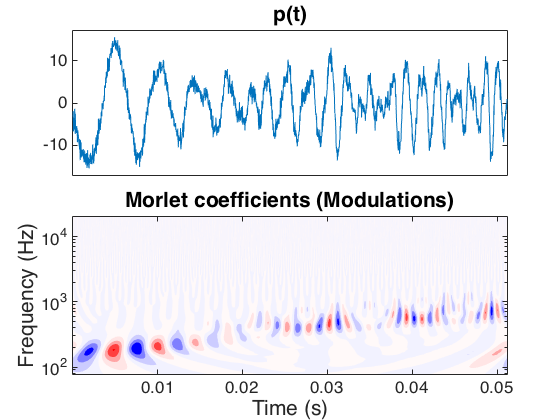
\includegraphics[width=.5\textwidth]{Morlet_real.png}
    \caption{Here goes the caption}
    \label{f:example}
\end{figure}

% \input{./Chapters/Chapter2}
% \input{./Chapters/Chapter3}
% \input{./Chapters/Chapter4}
% \input{./Chapters/Chapter5}

%------------------------------------------------------------------------
%	THESIS CONTENT - APPENDICES
%------------------------------------------------------------------------
\appendix % Cue to tell LaTeX that the following 'chapters' are Appendices
% Appendix Template

\chapter{Appendix Title Here} % Main appendix title

\label{AppendixX} % Change X to a consecutive letter; for referencing this appendix elsewhere, use \ref{AppendixX}

%\lhead{Appendix X. \emph{Appendix Title Here}} % Change X to a consecutive letter; this is for the header on each page - perhaps a shortened title
% \input{./Appendices/AppendixB}
% \input{./Appendices/AppendixC}

%------------------------------------------------------------------------
%	BIBLIOGRAPHY
%------------------------------------------------------------------------
\backmatter
\setstretch{1.2}
\addcontentsline{toc}{chapter}{References} % Add the "Abstract" page entry to the Contents
\bibliographystyle{acm} % Use the "acm" (or "unsrtnat", etc.) BibTeX style for formatting the Bibliography; acm forces the alphebetical ordering & abbreviated author names & journals - no need to manually change each reference
\bibliography{./references} % The references (bibliography) information are stored in the file named "references.bib"
\clearpage % Start a new page

%------------------------------------------------------------------------
%	VITA
%------------------------------------------------------------------------
\addcontentsline{toc}{chapter}{Vita} % Add the "Abstract" page entry to the Contents
\setboolean{@twoside}{false}
% include the resume page, as required by the graduate school
%\includepdf[pages=-, offset=75 -75]{resume.pdf}



\end{document}